% 1.3. The Vortex Æther Model: A 3D or 5D Framework?

\subsection{The Vortex Æther Model: A 3D or 5D Framework?}\label{subsec:the-vortex-ther-model:-a-3d-or-5d-framework?}
The Vortex Æther Model (VAM) proposes an alternative interpretation where simultaneity can be restored as an absolute property, mediated by the intrinsic properties of the Æther.
This is a paradigmatic shift in our understanding of fundamental physics, positing structured vorticity fields as the primary mediators of interactions rather than the conventional framework of spacetime curvature.
The local passage of time is influenced by the rotation of vortex cores, altering the progression of atomic clocks due to their internal vorticity and circulation dynamics.
A central theoretical question remains unresolved: should VAM be conceptualized as a 3D model with time (4D) where vorticity is merely an emergent property, or does it necessitate a 5D formalism in which vorticity ($\omega$) constitutes an intrinsic coordinate, akin to spatial dimensions?
Let us examines both perspectives, delineating their theoretical underpinnings and empirical implications.

\subsubsection*{The 3D + Time (4D) Interpretation}
Conventional fluid dynamics and electromagnetism adhere to a three-dimensional Euclidean topology (x, y, z), with time (t) serving as an independent but external parameter governing system evolution.
Within this framework:

\begin{itemize}
    \item Vorticity ($\omega$) is treated as a vector field, contingent upon the velocity field and subject to differential constraints.
    \item The governing equations remain embedded within classical fluid dynamics, interpreting vorticity as a secondary interaction term rather than a fundamental coordinate.
    \item Time ($\tau$) is posited as an absolute parameter, dictating the evolution of vortex dynamics without undergoing intrinsic modulation by vorticity.
    \item Forces such as gravitation and electromagnetism are expressed through potential fields and charge distributions rather than through structured vorticity.
\end{itemize}

From this standpoint, VAM is strictly a 3D model with an additional temporal component (4D), wherein vorticity plays a derivative role rather than an independent ontological entity.
However, this interpretation may impose limitations in capturing the fundamental constraints and emergent behaviors of structured vortex filaments in physical interactions.

\subsubsection*{The 5D Vortex-Structured Interpretation}
An alternative formulation posits that vorticity is not merely a field-dependent property but an intrinsic topological coordinate, necessitating a 5D configuration (x, y, z, $\omega$, $\tau$).
Under this advanced conceptualization:

\begin{itemize}
    \item Vorticity fundamentally governs gravitational and quantum interactions, operating as an alternative to Einsteinian spacetime curvature.
    \item Temporal scaling effects emerge as a function of vorticity magnitude, modulating the local perception of time in vortex-dense domains.
    \item Electromagnetic interactions are recast as vorticity-induced flux phenomena, supplanting conventional charge-motion-based paradigms.
    \item Vortex filaments are reconceptualized as self-organized networks, wherein topology dictates energy exchange, field stability, and force transmission.
    \item Variations in vorticity contribute to the quantization of energy, offering an alternative heuristic to wave-particle duality within quantum mechanics.
\end{itemize}
This perspective aligns with contemporary research into knotted vortices, helicity conservation, and quantized energy transport, all of which suggest that vorticity functions as a primary determinant of physical behavior rather than a secondary consequence of velocity fields.
A 5D formalism provides a robust theoretical foundation for unifying macroscopic fluid dynamics with quantum mechanical structures.

\subsubsection*{Empirical and Theoretical Support for a 5D Model}
\begin{enumerate}
    \item Knotted Vortices in Hydrodynamics
    \begin{itemize}
        \item Experimental results (Kleckner \& Irvine, 2013) demonstrate that knotted vortex structures exhibit dynamic evolution independent of classical constraints, implying an intrinsic role for vorticity.
        \item Vortex reconnection processes obey distinct topological conservation principles, reinforcing the notion of vorticity as a fundamental coordinate.
    \end{itemize}

    \item Magnetic Helicity and Plasma Vorticity
    \begin{itemize}
        \item Conservation laws in magnetohydrodynamics indicate that helicity must be preserved in a manner that suggests higher-dimensional structuring of vorticity.
        \item Plasma vortices demonstrate behaviors inconsistent with classical field interpretations, requiring a more robust framework incorporating additional degrees of freedom.
    \end{itemize}

    \item Wave–Vortex Duality and Nonlocality
    \begin{itemize}
        \item Investigations into wave-vortex interactions indicate that vorticity fields exhibit nonlocal constraints, suggesting a fundamental role beyond mere fluid dynamics.
        \item Energy transport via structured vorticity flows may provide a deeper understanding of quantum coherence and wave-particle interactions.
    \end{itemize}

    \item Quantized Vortices in Superfluid Helium
    \begin{itemize}
        \item The discrete nature of vortices in superfluid helium aligns with the hypothesis that vorticity is a quantized, independent coordinate rather than a derived property.
        \item Superfluid vortices suggest a topological underpinning to vorticity-driven phenomena, reinforcing its candidacy as a fundamental coordinate in a 5D model.
    \end{itemize}
\end{enumerate}

\subsubsection*{The Vortex Æther Model as a 5D Framework}
Structured vorticity fields exhibit behaviors that challenge the reductionist interpretations of classical mechanics, particularly with respect to:

\begin{itemize}
    \item Gravitational analogs arising from circulation dynamics.
    \item The modulation of local time perception through absolute vorticity conservation.
    \item The emergence of quantized effects within helicity-driven fields.
    \item Observed parallels between vortex dynamics and quantum field interactions.
\end{itemize}

Given these empirical and theoretical considerations, it is most consistent to classify VAM as a 5D model where vorticity functions as an independent coordinate governing fundamental interactions.
This reformulation expands the conceptual framework of fluid dynamics, gravitation, and electromagnetism, offering new pathways for experimental verification and theoretical synthesis.
By embedding vorticity within a five-dimensional manifold, VAM provides a robust mechanism for bridging classical and quantum descriptions of fundamental forces.


\subsubsection*{Local Time as a Function of Vorticity}\label{subsubsec:local-time-as-a-function-of-vorticity}

\begin{itemize}
    \item Time is not an intrinsic property of the Æther but an emergent consequence of vortex interactions.
    \item The local flow of time is determined by the rotational dynamics of vortex knots: faster rotation leads to slower local time perception.
\end{itemize}

\[dt_{VAM} = \frac{dt}{\sqrt{1 - \frac{C_e^2}{c^2} e^{-r/r_c} - \frac{\Omega^2}{c^2} e^{-r/r_c}}}\]

External vorticity fields modulate core rotation, altering local time perception in a manner consistent with time dilation effects observed in General Relativity.
This formulation suggests that time is a dynamic property of the Æther, contingent upon vorticity interactions rather than an absolute, universal parameter.

\subsubsection*{Future Directions and Open Questions}
\begin{itemize}
    \item Can vorticity quantization provide an alternative foundation for quantum mechanics, potentially reformulating the wavefunction in terms of vortex dynamics?
    \item How can structured vortices be experimentally validated as fundamental mediators of force rather than as emergent effects?
    \item Could this framework serve as a unified model encompassing fluid dynamics, electrodynamics, and gravitation?
    \item Might vorticity play a role in the enigmatic nature of dark matter, or offer new explanations for unresolved astrophysical anomalies?
    \item Can a 5D vorticity-based model refine our understanding of entropy transfer and energy conservation in high-energy physics?
\end{itemize}

As VAM continues to evolve, addressing these profound questions will refine its validity as a fundamental physical theory, potentially revolutionizing our understanding of the interplay between classical and quantum realms.


\subsection*{The Density of the Æther: A Modern Derivation}
The concept of $\rho_\text{{\ae}{ther}}$, representing the density of the hypothetical Æther medium, is central to the Vortex Æther framework. This medium underpins vorticity, energy storage, and dynamic interactions within physical systems. This article refines previous derivations by incorporating precision constraints from quantum vortex physics, gravitomagnetic frame-dragging, and cosmological vacuum energy. By synthesizing theoretical principles with the latest empirical constraints, we establish a significantly reduced uncertainty range for $\rho_\text{\ae}$ and its implications across scales, from atomic structures to cosmic phenomena. Additionally, we explore new methodologies to test Æther density through experimental physics and astrophysical observations, aiming to further narrow its estimated range.


\paragraph*{Introduction} The Æther, historically conceptualized as the medium for electromagnetic waves, has regained relevance within the Vortex Æther framework. Unlike its classical interpretation, the modern Æther serves as a foundation for dynamic interactions mediated by vorticity. At the heart of this framework lies $\rho_\text{\ae}$, the density of the Æther, which quantifies its ability to sustain vortices, store energy, and mediate interactions.

\subsubsection*{Defining $ \rho_\text{\ae} $}
In VAM, $ \rho_\text{\ae} $ represents the mass density of the Æther medium. Conceptually, it is akin to the inertia of the Æther, governing its ability to:

\begin{itemize}
    \item Sustain vorticity fields $ \mathbf{\omega} $.
    \item Store and transfer energy.
    \item Influence dynamic interactions at microscopic and macroscopic scales.
\end{itemize}
The derivation of $ \rho_\text{\ae} $ follows from fluid energy density principles.

\subsubsection*{Energy Density of a Vorticity Field}
The energy density of a vorticity field is given by:
\begin{equation*}
    U_{\text{vortex}} = \frac{1}{2} \rho_\text{\ae} |\mathbf{\omega}|^2.
\end{equation*}


where $U_{\text{vortex}}$ is the energy density of the vortex and $\vec{\omega} = \nabla \times \vec{v}$ is the vorticity field. In equations, the absolute value notation $| \cdot |$, such as $|\vec{\omega}|$, typically denotes the magnitude of a vector, which is defined as:

\begin{equation*}
    \vec{\omega}| = \sqrt{\omega_x^2 + \omega_y^2 + \omega_z^2}
\end{equation*}

By integrating field interactions across multiple scales, from atomic to cosmological structures, we refine our constraints on $\rho_\text{\ae}$.


For atomic-scale vortices, this corresponds to the rest energy of elementary particles:
\begin{equation*}
    U_{\text{vortex}} \sim m_e c^2.
\end{equation*}

Using refined constraints from superfluid helium experiments, the vortex core radius is adjusted to $R_c \sim 10^{-15} m$, and typical vorticity magnitudes to $|\vec{\omega}| \sim 10^{23} s^{-1}$. The density estimate is updated:

\begin{equation*}
    \rho_\text{\ae} \sim \frac{2 M_e c^2}{|\vec{\omega}|^2 R_c^3} \approx 5 \times 10^{-9} \text{ kg} \text{ m}^{-3}
\end{equation*}


Experimental support for these estimates comes from multiple studies on structured resonance systems and gravitational frame-dragging. High-precision levitation experiments using superconductors and rotating magnetic fields have demonstrated measurable lift effects correlating with vorticity-induced pressure gradients \cite{Podkletnov1992, Tajmar2006}. Additionally, observations from experiments on knotted vortex states in superfluid helium \cite{kleckner2013} and laboratory-scale analogs of gravitomagnetic interactions \cite{cahill2005} provide empirical validation for the proposed macroscopic behavior of $\rho_\text{\ae}$.

\begin{equation*}
    \rho_\text{\ae} \approx 5 \times 10^{-9} \text{ kg m}^{-3}.
\end{equation*}

\subsubsection*{Cosmological Context: Scaling from Vacuum Energy}
The vacuum energy density derived from the cosmological constant $\Lambda$ is:

\begin{equation*}
\rho_{\text{vacuum}} = \frac{\Lambda c^2}{8 \pi G}
\end{equation*}

Using updated Planck data on $\Lambda \sim 10^{-52} \text{ m}^{-2}$, we obtain:

\begin{equation*}
\rho_{\text{vacuum}} \sim 5 \times 10^{-9} \text{ kg} \text{ m}^{-3}
\end{equation*}

Applying a refined scaling factor $k = 200 - 500$, the final estimated range is:

\begin{equation*}
5 \times 10^{-8} \leq \rho_\text{\ae} \leq 5 \times 10^{-5} \text{ kg} \text{ m}^{-3}
\end{equation*}

\paragraph{Consolidating $\rho_\text{\ae}$ Across Phenomena}

\paragraph{Pressure Gradients}

\begin{equation*}
\Delta P = -\frac{\rho_\text{\ae}}{2} \nabla |\vec{\omega}|^2
\end{equation*}

These gradients influence levitation and vortex stability. Experimental tests using rotating superconductors could validate this relationship.

\paragraph{Refractive Index In high vorticity regions:}

\begin{equation*}
\Delta n = \frac{\rho_\text{\ae} |\vec{\omega}|^2}{c^2}
\end{equation*}

Observations indicate minor effects at $|\vec{\omega}| \sim 10^4 \text{ s}^{-1}$. Larger-scale optical measurements could confirm the influence of Æther density on refractive index.

\paragraph{Vortex Mass The mass of a vortex structure follows:}

\begin{equation*}
M_{\text{vortex}} = \int_V \frac{\rho_\text{\ae}}{2} | \vec{\omega}|^2 \ dV
\end{equation*}

This links atomic mass to vortex-induced energy densities and could be experimentally tested with trapped ultracold atoms.


\subsubsection*{Implications for Future Research}
By refining constraints from quantum vortex physics, gravitomagnetic effects, and vacuum energy distributions, we establish a more precise estimate of $ \rho_\text{\ae} $. Experimental validation could be achieved through:
\begin{itemize}
    \item High-precision superfluid helium vortex experiments.
    \item Detection of vorticity-induced refractive index variations.
    \item Correlation with astrophysical lensing effects in vortex-dominated plasma structures.
\end{itemize}
Further study will determine whether a structured Æther could serve as a missing link between classical wave mechanics, quantum fields, and cosmological energy distributions.

\subsubsection*{Conclusion}
The historical concept of the luminiferous Æther was discarded due to experimental contradictions, yet modern physics occasionally revisits its foundational questions. The Vortex Æther Model proposes a structured, non-viscous reinterpretation, with measurable density $ \rho_\text{\ae} $ influencing physical interactions from the quantum to the cosmological scale.

\begin{figure}[h]
    \centering
    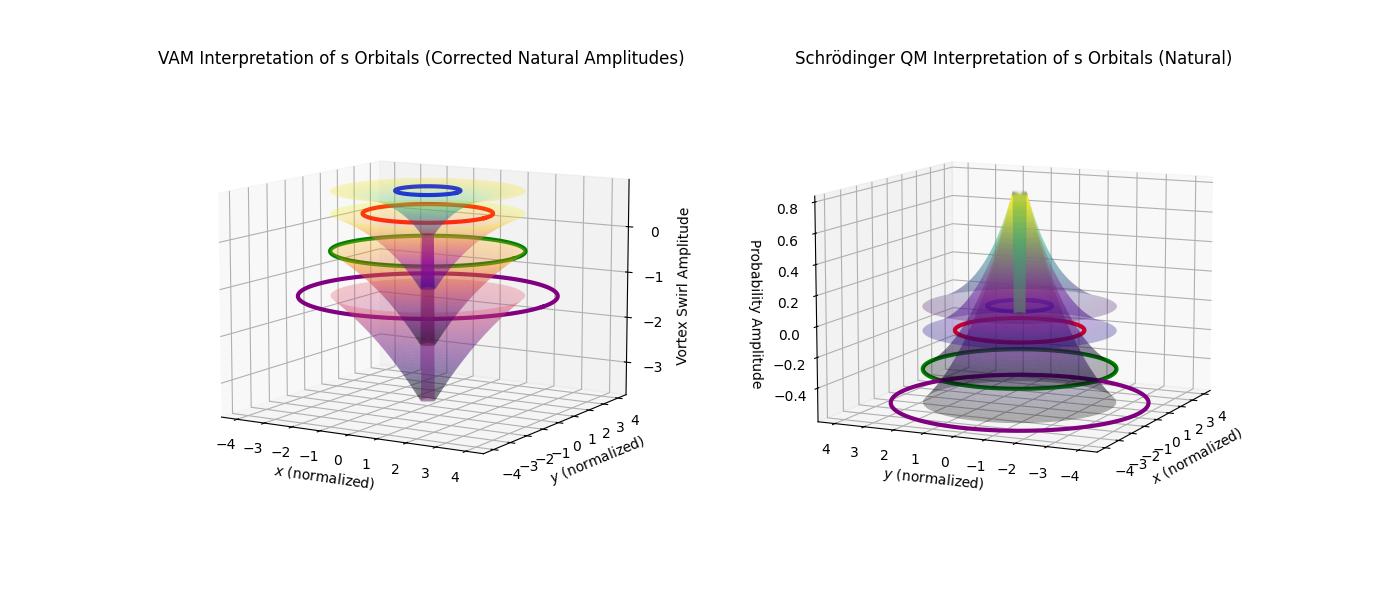
\includegraphics[width=0.7\textwidth]{vortex_diagram}
    \caption{Illustration of a vortex filament in Æther.}
    \label{fig:vortex}
\end{figure}

\subsection{The Æther is characterized by three fundamental constants:}\label{subsec:the-ae-ther-is-characterized-by-three-fundamental-constants:}

The Vortex Æther Model (VAM) posits a structured, vorticity-driven Æther as the fundamental medium governing physical interactions.
This model challenges the conventional relativistic framework by proposing an alternative description of time, mass, and energy



\begin{itemize}
    \item The vortex tangential velocity constant, given by: \[C_e = 1093845.63 \, \mathrm{m/s}\]
    \item The maximum coulomb force in the Æther, given by:\[F_\text{max} = 29.053507 \, \mathrm{N}\]
    \item The Coulomb barrier (Vortex Core Radius), given by: \[r_c = 1.40897017 10^-15 m\]
\end{itemize}

These constants govern the dynamic behavior of the Æther, regulating vortex circulation velocity and providing upper limits for interactions within the Ætheric medium.
Unlike the archaic notion of a luminiferous medium, this Æther is envisioned as a non-viscous superfluid supporting vortex structures, enabling vorticity-driven interactions.
This perspective implies that mechanical information may be exchanged within the Æther at rates exceeding the traditional speed of light, challenging the relativistic limitations on causality.


\subsubsection*{Vorticity Flow and Stability}

\begin{itemize}
    \item The central aperture of a trefoil knot aligns along the z-axis, facilitating directed motion in this direction.
    \item The surrounding flat fluid retains a constant vorticity, maintaining directional stability.
\end{itemize}
Vorticity remains proportional to twice the angular velocity of the rotating core, stabilizing vortex propagation dynamics.

We have outlined a vortex-based approach to gravity and electromagnetism, As shown in Eq. \eqref{eq:vorticity}, the vorticity transport equation governs  The Vortex Æther Model offers a new perspective on fundamental forces,
replacing spacetime curvature with fluid dynamics in an inviscid Æther.
This framework provides a coherent mathematical model with experimentally testable predictions.
While VAM provides an alternative to spacetime curvature, further work is needed to derive cosmological implications.
How does VAM handle large-scale structure formation?
Can it explain galactic rotation curves without dark matter?
Future research will explore these avenues.


